\chapter{Digitalización}
% ----------------------

\label{C:Digitalización y control}

\section{Principio de Digitalización}
La implementación del control digital es el punto principal de este proyecto, por lo que 
En la figura~\ref{F:estructura_archivos} se puede ver la estructura de archivos. En la carpeta \entreComillas{contenido}, se encuentran los archivos que componen cada capítulo del informe; en \entreComillas{apéndices}, se encuentran los apéndices; en \entreComillas{imagenes}, las imágenes y gráficos utilizados, sea el formato que sea, \texttt{.png}, \texttt{.jpg}, \texttt{.pdf}, o cualquier otro; en \entreComillas{bibliografia} se encuentra el archivo \texttt{bibliografia.bib}, donde están especificadas todas las referencias utilizadas en el informe; y en \entreComillas{codigo}, se encuentra el código fuente de programas que se hayan incluido al informe.

\begin{figure}
    \centering
    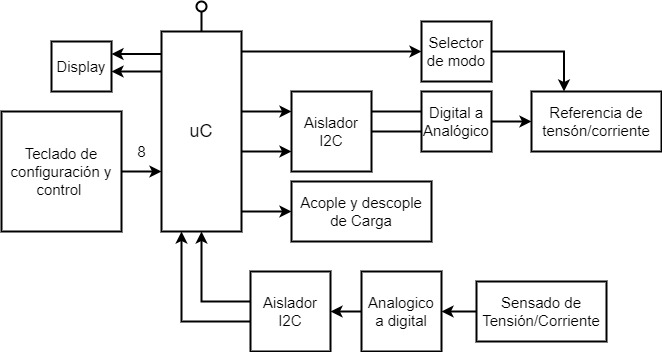
\includegraphics[scale=0.8]{./imagenes/digitaldigital.jpg}
    \caption{Estructura de archivos de la plantilla.}
    \label{F:estructura_archivos}
\end{figure}

\subsection{Datos generales}
Los datos de la portada y la página de aprobación se ingresan en \texttt{proyecto.tex}. A continuación, se muestra exactamente donde se deben ingresar los datos.

\lipsum[5-6]


